\documentclass[10pt]{report}
\usepackage{times}
\usepackage{anysize}
\usepackage{multicol}
\usepackage{fancyhdr}
\usepackage{graphicx}
\usepackage{amsmath}

\setlength{\headheight}{15.2pt}
\setlength{\headwidth}{495pt}
\setlength{\parindent}{0pt}
\setlength{\parskip}{1em}
\pagestyle{fancy}
\rhead{Page \thepage}
\lhead{COMP3130 Othello Project}
\marginsize{2cm}{1.5cm}{2cm}{2cm}

\newenvironment{packed_enum}{
\begin{enumerate}
  \setlength{\itemsep}{0pt}
  \setlength{\parskip}{0pt}
  \setlength{\parsep}{0pt}
}{\end{enumerate}}

\begin{document}

\date{June 8th, 2012}
\title{Team Reverwesome: Othello Bot Project}
\author{Josh Godsiff, Jarrah Bloomfield}
\maketitle

\section*{\emph{Problem Outline}}
\hrule
    \begin{itemize}
  \item
    Modified Othello Game
  \item
    4 randomly removed squares
  \item
    10x10 board rather than the traditional 8x8
  \item
    Network communication with server
  \item
    150 seconds total time per player
  \item
    Design an agent to play intelligently
  \end{itemize}

\section*{\emph{Solution Outline}}
\hrule
    \begin{itemize}
  \item
    Static evaluation function based on feature weights
  \item
    Temporal Difference Learning
  \item
    Negamax search with alpha beta pruning
  \item
    Concurrent searching
  \item
    Time management
  \item
    C++ and Ada interfacing
  \end{itemize}

\section*{\emph{Static Evaluation}}
\hrule
    \begin{itemize}
  \item
    Use features weights to evaluate value of board states
  \item
    3 different feature sets - mention transitions
  \item
    15 weights for each piece position
	\begin{itemize}
		\item based on (naive) 8-way symmetry
		\item in actuality, only a 4-way symmetry exists. However, in practice this doesn't make a lot of difference.
		% Include picture showing the difference?
	\end{itemize}
  \item
    Weight for mobility - number of moves if it was our turn
  \item
   Weight for stability - number of stable pieces we own
  \item
   Weight for internals - number of internal pieces we own
  \end{itemize}

\section*{\emph{\textmd{Piece Stability}}}
\hrule
    \begin{itemize}
  \item
  Stability is the inability for a piece to ever be flipped. For example, corners are always stable.
  \item
   All 4 lines must be stable in one direction
  \item
   Line stability from the whole line being 'full'
  \item
   Line stability from the whole direction being stable and full in your favour
  \item
    Because of the removed squares, piece stability became especially important ahead
  \item
    Expensive check, but memory is used. false negatives on update function.
  \item
    Importance gets diluted in late game because in late game, EVERYTHING is stable. this is a consequence of only using 3 phases
  \end{itemize}

\begin{center}
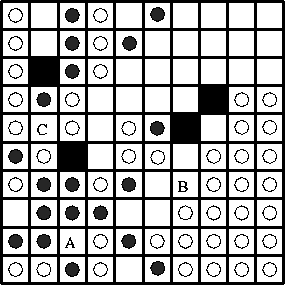
\includegraphics[scale=0.50]{stability.PNG}\\
Stable positions for white
\end{center}

\section*{\emph{\textmd{Mobility}}}
\hrule
    \begin{itemize}
  \item
	Mobility is a measure of the number of moves a player has in a given board state.
  \item
	High mobility tends to be much more important in the early to mid game than the number of pieces a player has, since Reversi boards can change very quickly.
  \item
	Much less useful in the later game, where we want to focus on pieces and stability.
  \item
	Has the unfortunate side-effect of making the branching factor quite large, meaning we cannot search to great depth.
  \end{itemize}

\section*{\emph{\textmd{Piece Internality}}}
\hrule
    \begin{itemize}
  \item
  A piece is internal if it has no empty neighbours
  \item
   Harder to dislodge, can result in higher mobility
  \item
   Cheap to check, partial memory used
  \end{itemize}

\section*{\emph{Temporal Difference Learning}}
\hrule
   \begin{itemize}
  \item
  	Used a fairly standard TD($\lambda$) policy.
  \item
	Play whole game, recieve reward $r\in \left\{1,0,-1 \right\}$ for win/draw/loss.
  \item
	For each board $b_k$ position in the game, find the direction to adjust the weight in, based on making a small change and seeing if it improves/worsens the result.
 \item
	Then run through all of it is successors, and calculate the weighted difference between it's value and the successor's.
  \item
	$\sum_{t=k}^T \lambda^t \left ( V(b_t) - V(b_k) + feedback \right)$
  \end{itemize}

\section*{\emph{\textmd{Learning Strategies}}}
\hrule
\begin{itemize}
	\item $\alpha = 0.0001$
		\\ Learning weight. Tend to get divergence if we set it any higher.
	
	\item $\epsilon = 0.15$
		\\ Used for $\epsilon$-greedy policy. The chance we'll pick a random move instead of a good one.
	\item $\gamma = 0.9$
		\\ Discount factor on how much we weight boards far into the 'future' when training.
		\\ Scales as $\gamma^t$, where $t$ is the number of boards in the futre we're looking.
	\end{itemize}

\section*{\emph{Negamax with alpha beta pruning}}
\hrule
    \begin{itemize}
  \item
    Adversarial search algorithm
  \item
    Minmax algorithm modified to negate the value at each step
  \item
    Attempts to maximise reward against adversary who is actively minimising reward
  \item
   $\alpha$ - $\beta$ pruning cuts sections of the game tree that an opponent would never choose
  \end{itemize}

\section*{\emph{\textmd{Negamax features}}}
\hrule
    \begin{itemize}
  \item
    Search to a moderate depth if close to the start of the game
  \item
    Search to a deep depth if close to the end of the game
  \item
    Add depth if exploring along a forced move
  \item
    Use static evaluation feature weights to evaluate how far in our favour the board value is
  \item
    Terminals in our favour worth $\infty$, in opponent's favour worth $-\infty$.
  \item
    This means we avoid a loss at all costs, and take a win at all costs (for example wiping out a player early)
  \end{itemize}

\section*{\emph{Concurrency}}
\hrule
    \begin{itemize}
  \item
	Use concurrency to distribute MinMax search across multiple CPUs, thereby (hopefully) reducing the time taken for a search.
 \item
	Have to find a model of parallelism which balances putting processing time where it's needed vs overhead in communication between threads.
 \item
	We settled for a simplistic model - give each thread one of the 'top-level' MinMax nodes to search through. When it's done, give it another one.
 \item
	Has the downside that $\alpha \beta$ pruning data does not get updated until a thread finishes its node.
 \item
	Initial nodes can take more time than they otherwise might have.
 \item
	But still end up with an $O(n)$ speed up, where $n$ is the number of cores.
  \end{itemize}

\begin{center}
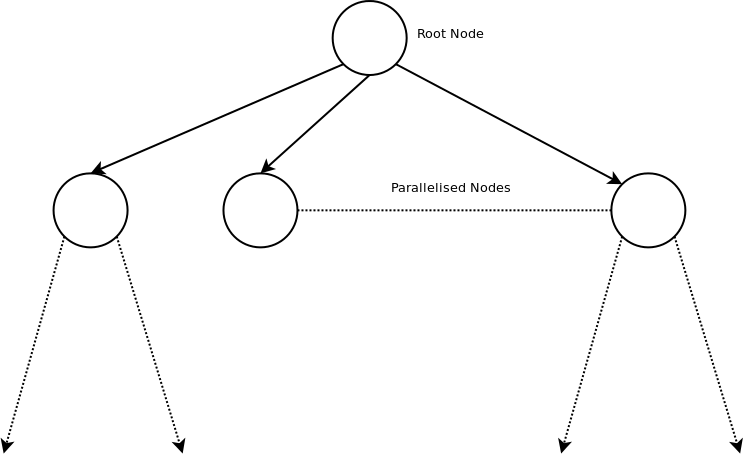
\includegraphics[scale=0.35]{concurrency.png}
\\Concurrency model
\end{center}

\section*{\emph{Time management}}
\hrule
    \begin{itemize}
  \item
    Vary the search depth depending on time left and how long the previous move took
  \item
     Below 5 seconds, drop to depth 2  
  \item
    Below 15 seconds, drop to depth 4
  \item
    If we have extra time, increase to 8
  \item
    If we have less time, decrease to 5
  \item
    Default to 7
  \end{itemize}

\section*{\emph{C++ and Ada}}
\hrule
    \begin{itemize}
  \item
    We took the C++ sample client code and used it to call procedures in Ada
  \item
    C++ client listened for new messages and saved them
  \item
   C++ called Ada procedures
  \item
   Procedures called entries on Ada's Main Task
  \item
   Messages and information passed using direct edits to shared memory
  \end{itemize}

\section*{\emph{\textmd{C++ and Ada Experiences}}}
\hrule
    \begin{itemize}
  \item
    Make the communication as simple as possible
  \item
   Don't call entries or complex data structures
  \item
   C++ decapitalises everything
  \item
   Avoid C++ and Ada running computation concurrently near shared data
  \item
   C++ and Ada store arrays in different fashions
  \end{itemize}

\section*{\emph{Other ideas (Monte Carlo)}}
\hrule
    \begin{itemize}
  \item
    	Use monte carlo prediction as a substitute for reward to help with learning of mid-game states
  \item
	Tends to make the algorithm learn more quickly, and on-the-fly
  \item
	Can also be used as a predictor of how good a board state is.
  \end{itemize}

\section*{\emph{Other ideas (MinMax)}}
\hrule
    \begin{itemize}
  \item
    Optimised search ordering - expand nodes by their value in our piece feature weights
  \item
	Store searches between moves. Could have saved a huge amount of computation time.
  \item
	Vary depth of search based on branching factor and volatility of the state.
  \end{itemize}

\section*{\emph{Other ideas (Evolutionary Algorithm)}}
\hrule
    \begin{itemize}
  \item
   	Use an evolutionary algorithm strategy to play agents off against each other.
  \item
	Use feature values as 'genes'.
  \item
	'Breeding' via exchanging features. Don't need a heuristic for which to exchange, as features tend to be relatively independent.
  \item
	Mutation via small random change to a feature.
	\\ e.g. from a uniform distribution around (-1,1), or
	\\ Normal distribution with mean 0.
  \item
	Essentially still doing gradient decent. Can be used as a substitute for an $\epsilon$-greedy policy.
  \end{itemize}

\section*{\emph{Other ideas (Utilising opponent time)}}
\hrule
    \begin{itemize}
  \item
   	Compute further down the game tree while the opponent is thinking
  \item
	Could allow significantly greater search depths to be reached
  \item
	Required memory management and large data structures
  \item
	Ada would be very well positioned to perform this task
  \end{itemize}

\end{document} 
